\documentclass[]{beamer}
% Class options include: notes, notesonly, handout, trans,
%                        hidesubsections, shadesubsections,
%                        inrow, blue, red, grey, brown

% Theme for beamer presentation.
\usepackage{beamerthemesplit} 
% Other themes include: beamerthemebars, beamerthemelined, 
%                       beamerthemetree, beamerthemetreebars  

\title{PHY115}    % Enter your title between curly braces
\author{Week2: Motion Along a Straight Line}                 % Enter your name between curly braces
\institute{Digipen}      % Enter your institute name between curly braces
\date{Spring 2021} 

\begin{document}

% Creates title page of slide show using above information
\begin{frame}
  \titlepage
\end{frame}
%\note{Talk for 30 minutes} % Add notes to yourself that will be displayed when
                           % typeset with the notes or notesonly class options

\section[]{}

% Creates table of contents slide incorporating
% all \section and \subsection commands
\begin{frame}
  \tableofcontents
\end{frame}

%%%%%%%%%%%%%%%%%%%%%%%%%%%%%%%%%%%%%%%%%%%%%%%%%%%%%%%%%%%%%%%%%%%
\section{Motion Along a Straight Line}
\subsection{Displacement, Time, and Average Velocity}

  

%%%%%%%%%%%%%%%%%%%%%%%%%%%%%%%%%%%%%%%%%%%%%%%%%%%%%%%%%%%%%%%%%%%
\begin{frame}

\begin{itemize}
\item  In this section we concentrate in the motion of a body moving
along a straight line.
\pause
\item  We introduce the physical quantities velocity and acceleration.
\pause
\item Both are vectors, they have magnitud and direction.
\end{itemize}
 
    

\end{frame}

%%%%%%%%%%%%%%%%%%%%%%%%%%%%%%%%%%%%%%%%%%%%%%%%%%%%%%%%%%%%%%%%%%%
\begin{frame}

Average Velocity
\vspace{3mm}

\begin{equation}
v_{av}=\frac{x_2-x_1}{t_2-t_1}=\frac{\Delta x}{\Delta t}
\end{equation}


  \begin{center}
  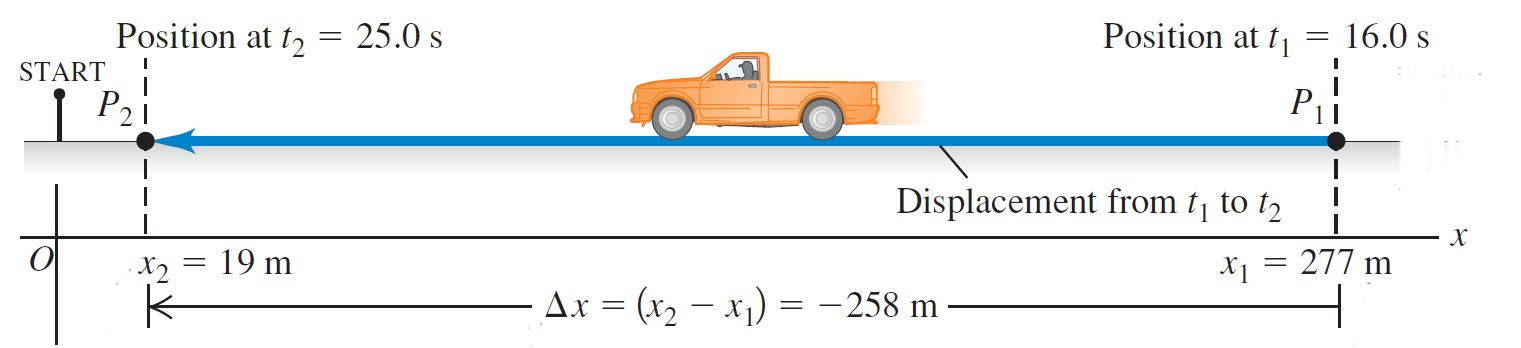
\includegraphics[height=1.in]{images/2.jpg}
\end{center}
 \end{frame}
    



%%%%%%%%%%%%%%%%%%%%%%%%%%%%%%%%%%%%%%%%%%%%%%%%%%%%%%%%%%%%%%%%%%%
\begin{frame}
Position as a function of time

   \begin{columns}[c]
   \column{2in}  % slides are 3in high by 5in wide
  
\begin{itemize}
\item We can represent the variation of the position respect to the time as a function: $x=x(t)$.
\pause
\item $x(t)$ \textit{Does not} represent the object’s path in space.
\pause
\item Even for a straight-line motion, $x(t)$ may not be a strigh line.
\end{itemize}



   \column{2.5in}
   
   \begin{figure}[h!]
 
  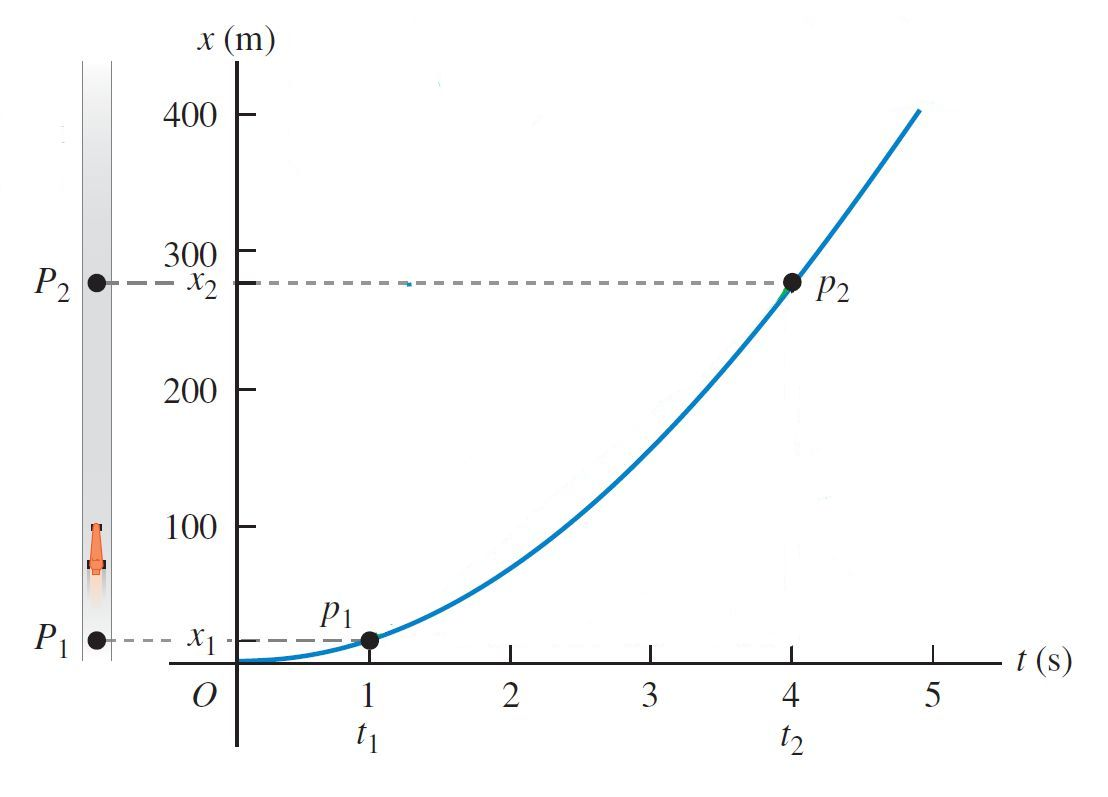
\includegraphics[width=1.\textwidth]{images/3.jpg}
   \caption{Position vs. time. {\tiny Figure from Sears and Zemansky's University Physics 
   with Modern Physics, 13th Edition.} }
\end{figure}



   \end{columns}




 \end{frame}


%%%%%%%%%%%%%%%%%%%%%%%%%%%%%%%%%%%%%%%%%%%%%%%%%%%%%%%%%%%%%%%%%%%
\begin{frame}
Plot of the average velocity

   \begin{columns}[c]
   \column{2in}  % slides are 3in high by 5in wide
  
\begin{itemize}
\item  The average velocity is the \textit{slope} of the line $p_1p_2$.
\item The average velocity depends only on the total displacement,
not on the details of what happens inbetween. 
\item If distance is given in $m$ and time in $s$, average velocity is measured
in $(m/s)$
\end{itemize}



   \column{2.5in}
   
   \begin{figure}[h!]
 
  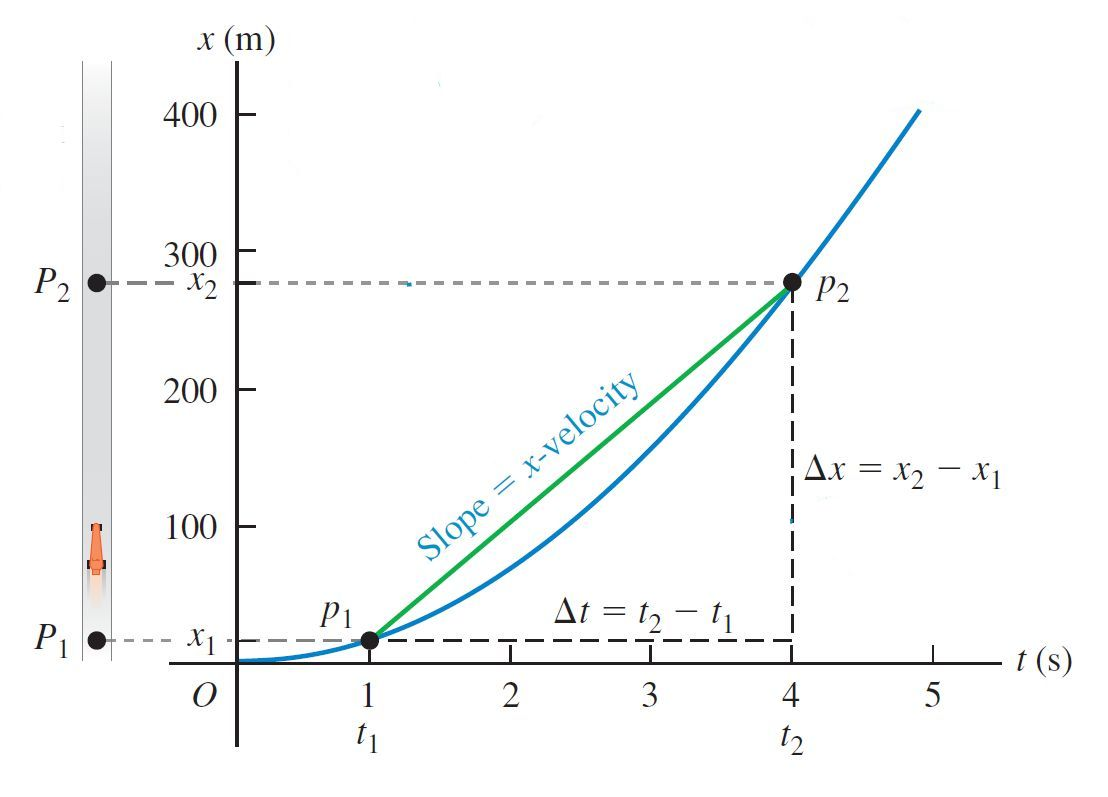
\includegraphics[width=1.\textwidth]{images/4.jpg}
   \caption{Position vs. time. {\tiny Figure from Sears and Zemansky's University Physics 
   with Modern Physics, 13th Edition.} }
\end{figure}



   \end{columns}




 \end{frame}



%%%%%%%%%%%%%%%%%%%%%%%%%%%%%%%%%%%%%%%%%%%%%%%%%%%%%%%%%%%%%%%%%%%
\begin{frame}
Test your understanding.

\vspace{3mm}

Each of the following automobile trips takes one hour.
The positive x-direction is to the east.  Rank the five trips in order of average velocity from most positive to most negative. 
  Which trips, if any, have the same average velocity? 
  For which trip, if any, is the average xvelocity equal to zero?

 
\begin{enumerate}
\item   Automobile A travels $50~km$ due east. 
\item  Automobile B travels $50~km$ due west. 
\item  Automobile C travels $60~km$ due east, then turns around and travels 10 km due west. 
\item  Automobile D travels $70~km$ due east. 
\item  Automobile E travels $20~km$ due west, then turns
around and travels $20~km$ due east. 

\end{enumerate}


 \end{frame}

%%%%%%%%%%%%%%%%%%%%%%%%%%%%%%%%%%%%%%%%%%%%%%%%%%%%%%%%%%%%%%%%%%%
\subsection{Instantaneous Velocity}
%%%%%%%%%%%%%%%%%%%%%%%%%%%%%%%%%%%%%%%%%%%%%%%%%%%%%%%%%%%%%%%%%%%
\begin{frame}
Instantaneous Velocity
\vspace{3mm}





   \begin{columns}[c]
   \column{2in}  % slides are 3in high by 5in wide
  
\begin{itemize}
\item  if we move the second point closer and closer to the first point
\item   the average velocity becomes the \textbf{instantaneous velocity} at point $p_1$.

\end{itemize}

\begin{equation*}
\boxed{v=\lim_{\Delta t\to0} \frac{\Delta x}{\Delta t}}
\end{equation*}


   \column{2.5in}
   
   \begin{figure}[h!]
 
  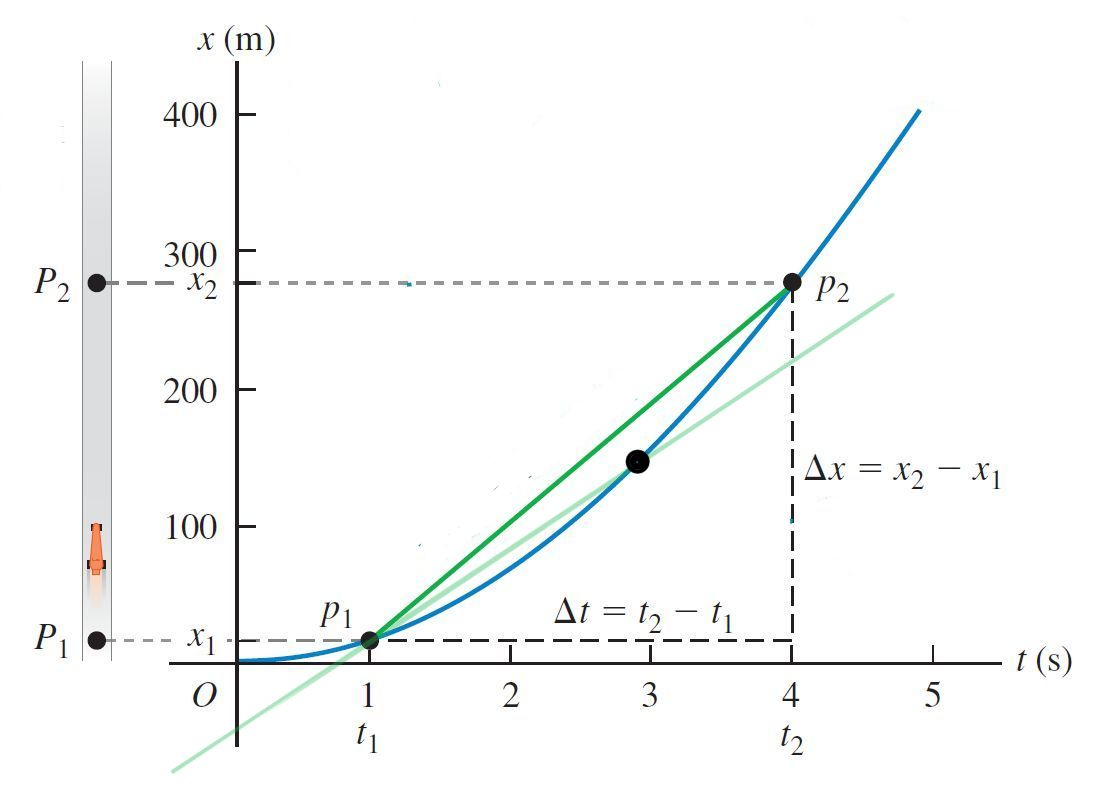
\includegraphics[width=1.\textwidth]{images/5.jpg}
   \caption{ {\tiny © University Physics 
   with Modern Physics, 13th Edition.} }
\end{figure}



   \end{columns}
   
   
   
   

 \end{frame}





%%%%%%%%%%%%%%%%%%%%%%%%%%%%%%%%%%%%%%%%%%%%%%%%%%%%%%%%%%%%%%%%%%%

\begin{frame}
Instantaneous Velocity
\vspace{3mm}
   \begin{columns}[c]
   \column{2in}  % slides are 3in high by 5in wide
  
\begin{itemize}
\item  if we move the second point closer and closer to the first point
\item   the average velocity becomes the \textbf{instantaneous velocity} at point $p_1$.

\end{itemize}

\begin{equation*}
\boxed{v=\lim_{\Delta t\to0} \frac{\Delta x}{\Delta t}}
\end{equation*}


   \column{2.5in}
   
   \begin{figure}[h!]
 
  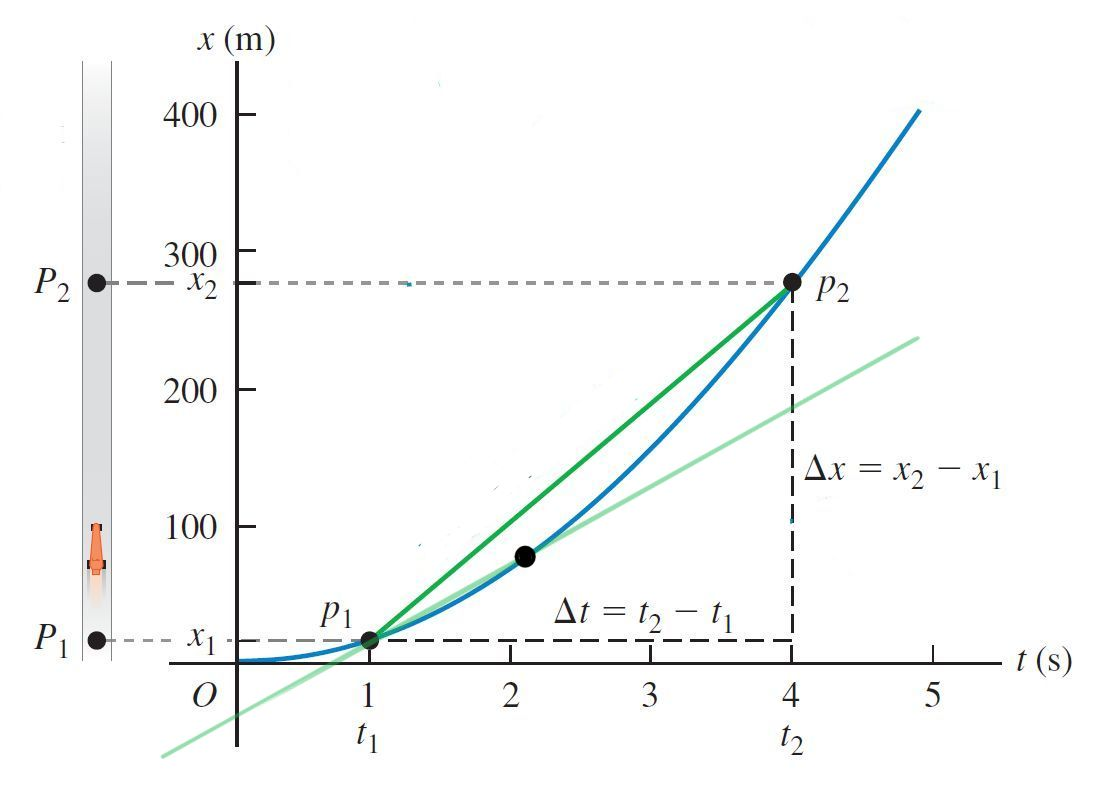
\includegraphics[width=1.\textwidth]{images/6.jpg}
   \caption{ {\tiny © University Physics 
   with Modern Physics, 13th Edition.} }
\end{figure}

   \end{columns}

 \end{frame}

%%%%%%%%%%%%%%%%%%%%%%%%%%%%%%%%%%%%%%%%%%%%%%%%%%%%%%%%%%%%%%%%%%%

\begin{frame}
Instantaneous Velocity
\vspace{3mm}
   \begin{columns}[c]
   \column{2in}  % slides are 3in high by 5in wide
  
\begin{itemize}
\item  if we move the second point closer and closer to the first point
\item   the average velocity becomes the \textbf{instantaneous velocity} at point $p_1$.

\end{itemize}

\begin{equation*}
\boxed{v=\lim_{\Delta t\to0} \frac{\Delta x}{\Delta t}}
\end{equation*}


   \column{2.5in}
   
   \begin{figure}[h!]
 
  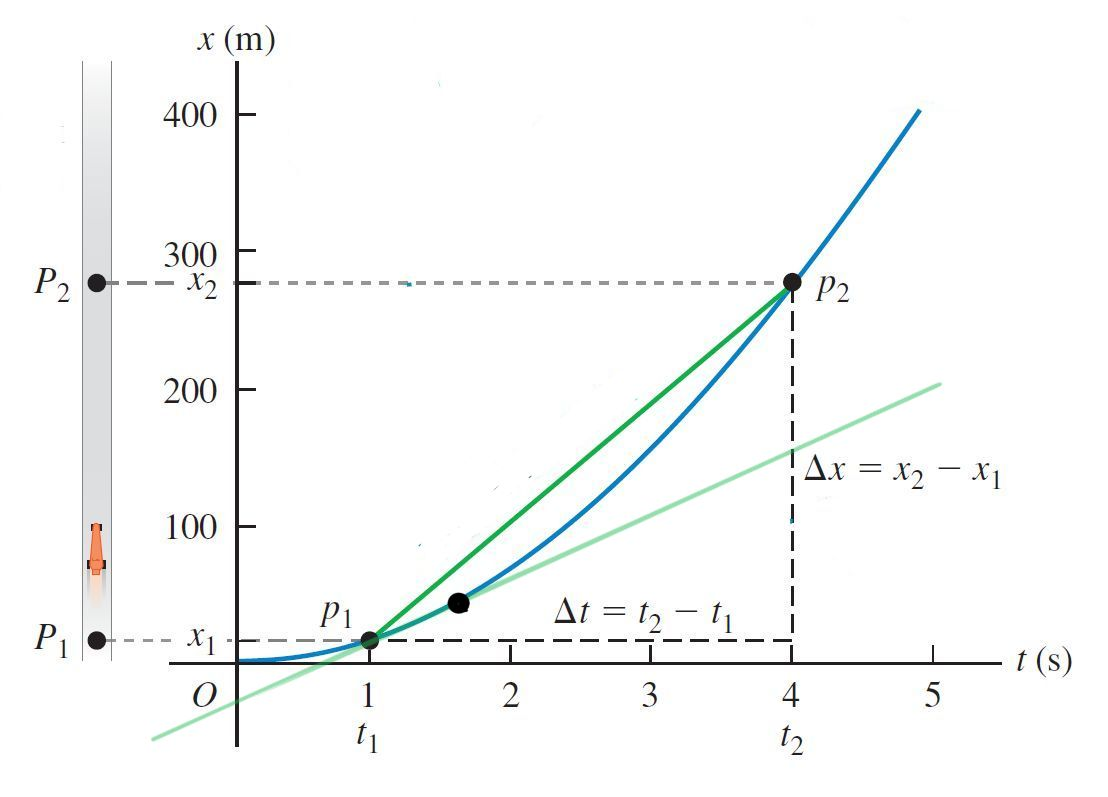
\includegraphics[width=1.\textwidth]{images/7.jpg}
   \caption{ {\tiny © University Physics 
   with Modern Physics, 13th Edition.} }
\end{figure}

   \end{columns}

 \end{frame}

%%%%%%%%%%%%%%%%%%%%%%%%%%%%%%%%%%%%%%%%%%%%%%%%%%%%%%%%%%%%%%%%%%%

\begin{frame}
Instantaneous Velocity
\vspace{3mm}
   \begin{columns}[c]
   \column{2in}  % slides are 3in high by 5in wide
  
\begin{itemize}
\item  if we move the second point closer and closer to the first point
\item   the average velocity becomes the \textbf{instantaneous velocity} at point $p_1$.

\end{itemize}

\begin{equation*}
\boxed{v=\lim_{\Delta t\to0} \frac{\Delta x}{\Delta t}}
\end{equation*}


   \column{2.5in}
   
   \begin{figure}[h!]
 
  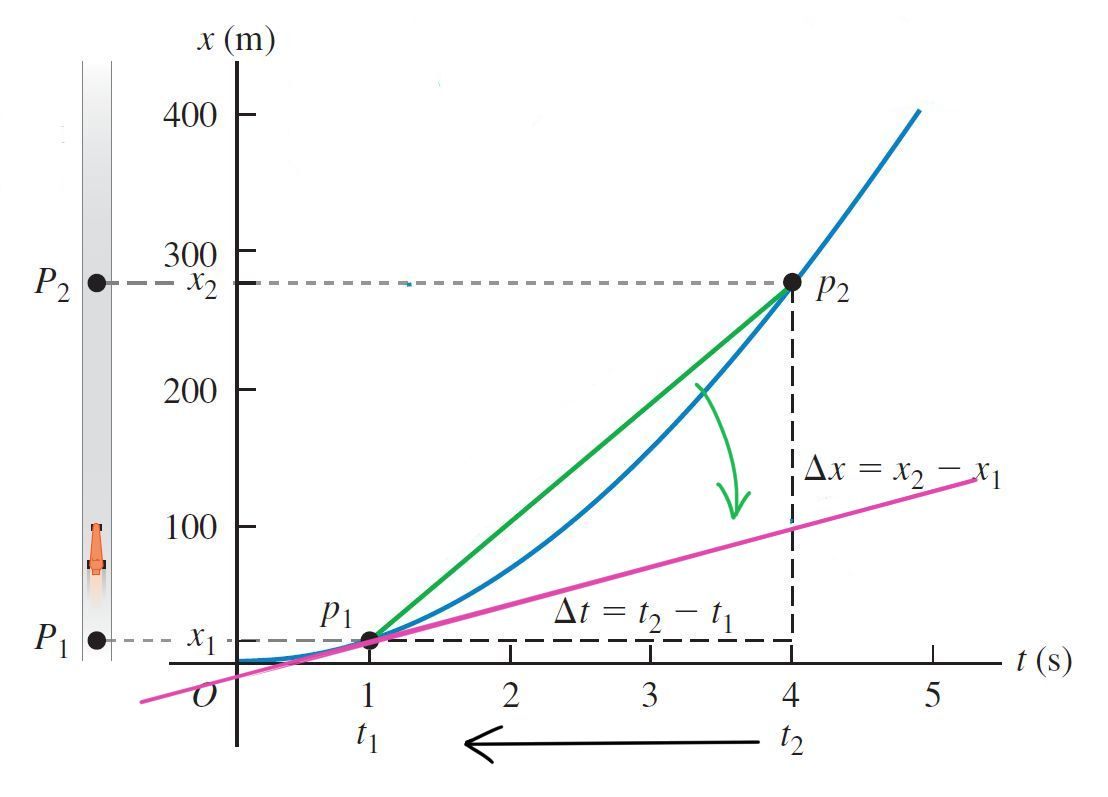
\includegraphics[width=1.\textwidth]{images/8.jpg}
   \caption{ {\tiny © University Physics 
   with Modern Physics, 13th Edition.} }
\end{figure}

   \end{columns}

 \end{frame}



%%%%%%%%%%%%%%%%%%%%%%%%%%%%%%%%%%%%%%%%%%%%%%%%%%%%%%%%%%%%%%%%%%%

\begin{frame}
\begin{itemize}
\item  The instantaneous velocity is a vector.
\pause
\item It has the same sign than $\Delta x$.
\pause
\item The instantanous speed is the magnitude of the instantaneous velocity.

\end{itemize}

 \end{frame}




%%%%%%%%%%%%%%%%%%%%%%%%%%%%%%%%%%%%%%%%%%%%%%%%%%%%%%%%%%%%%%%%%%%

\begin{frame}
CAUTION! 

\vspace{5mm}

The average  speed  is not the magnitude of the average  velocity.  
 \end{frame}



%%%%%%%%%%%%%%%%%%%%%%%%%%%%%%%%%%%%%%%%%%%%%%%%%%%%%%%%%%%%%%%%%%%

\begin{frame}
Finding Velocity on an x-t Graph
\vspace{3mm}

   
   \begin{itemize}
\item The isntantaneous velocity is the slope of the curve.

\end{itemize}
   
   \begin{figure}[h!]   
   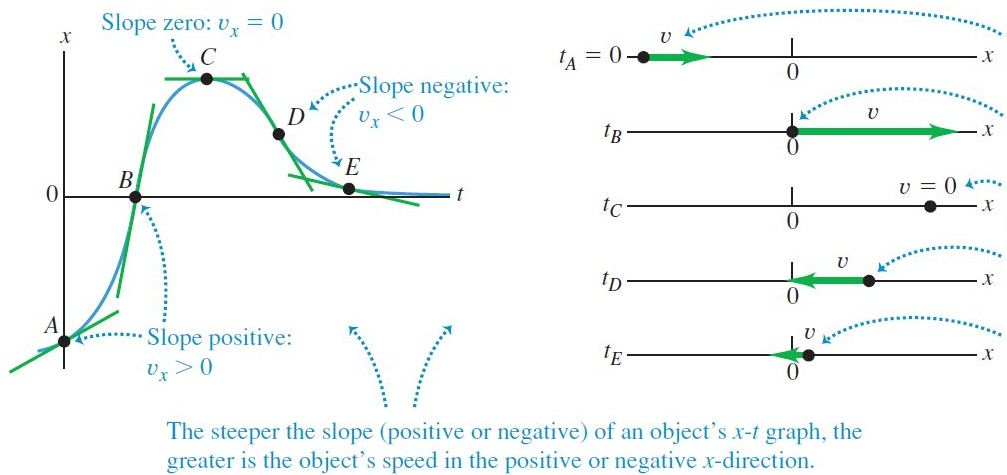
\includegraphics[width=1.\textwidth]{images/9.jpg}
   \caption{ {\tiny © University Physics 
   with Modern Physics, 13th Edition.} }
\end{figure}

 \end{frame}




%%%%%%%%%%%%%%%%%%%%%%%%%%%%%%%%%%%%%%%%%%%%%%%%%%%%%%%%%%%%%%%%%%%

\begin{frame}
Test your undertanding
\vspace{3mm}

The figure is an x-t graph of the motion of a particle.
   
 \begin{enumerate}
\item Rank the values of the particle’s velocity at the
points P, Q, R, and S from most positive to most negative.
\item At which points $v$ is positive? 
\item  At which points $v$ is negative? 
\item At which points $v$ is zero? 
\item Rank the values of the particle’s speed at the points P, Q, R, and S from fastest 
to slowest.

\end{enumerate}
   
   \begin{figure}[h!]   
   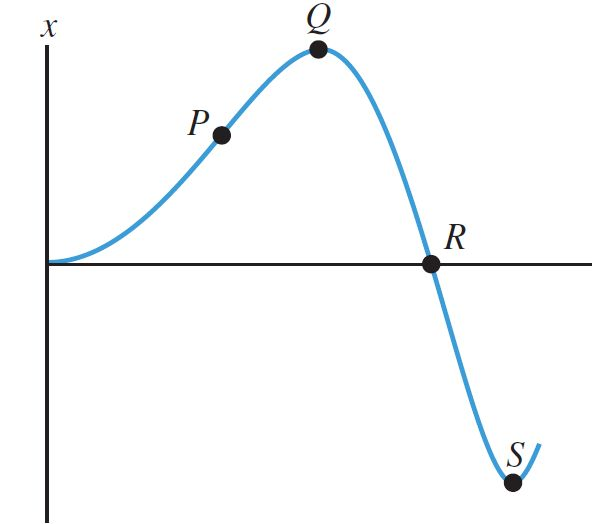
\includegraphics[width=0.4\textwidth]{images/10.jpg}
   \caption{ {\tiny © University Physics 
   with Modern Physics, 13th Edition.} }
\end{figure}

 \end{frame}



%%%%%%%%%%%%%%%%%%%%%%%%%%%%%%%%%%%%%%%%%%%%%%%%%%%%%%%%%%%%%%%%%%%

\begin{frame}

   \begin{columns}[c]
   \column{2in}  % slides are 3in high by 5in wide
  

When the velocity is constant, the average velocity is equal to the isntantaneous velocity.

\begin{equation}
v=\frac{\Delta x}{\Delta t}\rightarrow x(x)=vt+x_0
\end{equation}


   \column{2.5in}
   
   \begin{figure}[h!]
 
  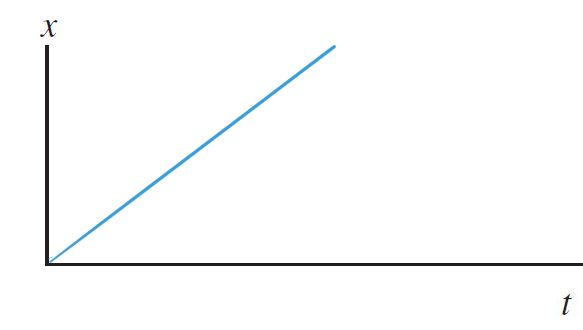
\includegraphics[width=1.\textwidth]{images/11.jpg}
  
\end{figure}

   \end{columns}





 \end{frame}



%%%%%%%%%%%%%%%%%%%%%%%%%%%%%%%%%%%%%%%%%%%%%%%%%%%%%%%%%%%%%%%%%%%




\begin{frame}

How is the velocity vs. time plot?





 \end{frame}


%%%%%%%%%%%%%%%%%%%%%%%%%%%%%%%%%%%%%%%%%%%%%%%%%%%%%%%%%%%%%%%%%%%
\subsection{Acceleration}
%%%%%%%%%%%%%%%%%%%%%%%%%%%%%%%%%%%%%%%%%%%%%%%%%%%%%%%%%%%%%%%%%%%



\begin{frame}

Average and Instantaneous Acceleration
\vspace{3mm}

\begin{itemize}  
\item The average acceleration is the change of the velocity in the time interval $\Delta t$
\end{itemize}

\pause
\begin{equation}
a_{av}=\frac{v_2-v_1}{t_2-t_1}=\frac{\Delta v}{\Delta t}
\end{equation}  
\pause


\begin{itemize}  
\item The instantaneous acceleration is the limit of the average velocity when $\Delta t \rightarrow 0$
\end{itemize}
\pause

\begin{equation}
a=\frac{d v}{d t}
\end{equation}

 \end{frame}



%%%%%%%%%%%%%%%%%%%%%%%%%%%%%%%%%%%%%%%%%%%%%%%%%%%%%%%%%%%%%%%%%%%




\begin{frame}

Finding Acceleration on a v-t Graph 
\vspace{3mm}

  \begin{figure}[h!]   
   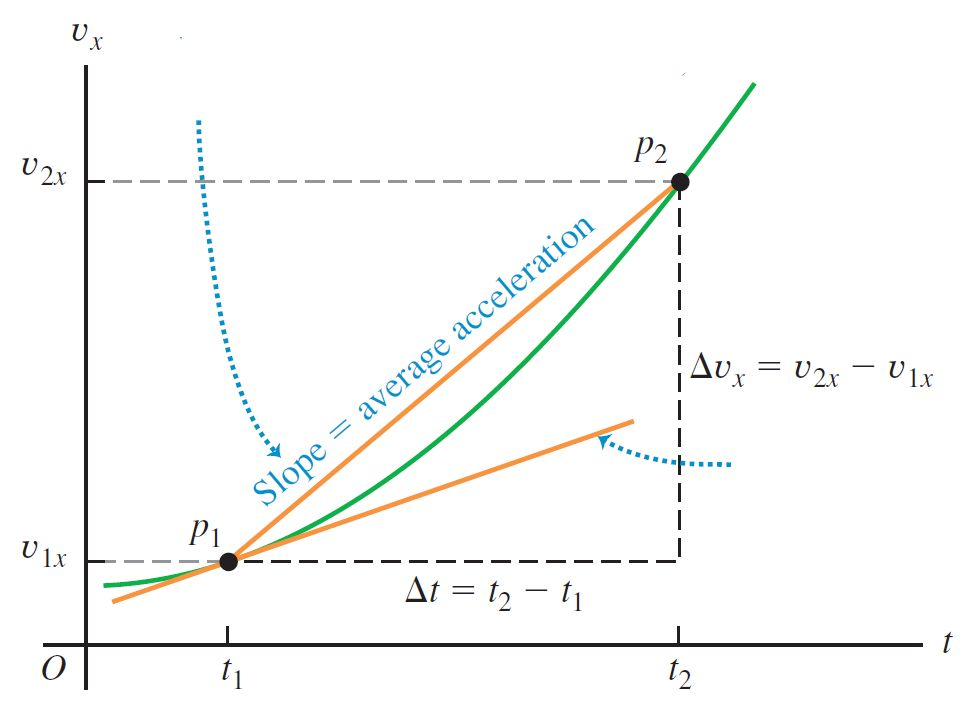
\includegraphics[width=0.8\textwidth]{images/12.jpg}
   \caption{ {\tiny © University Physics 
   with Modern Physics, 13th Edition.} }
\end{figure}

 \end{frame}






%%%%%%%%%%%%%%%%%%%%%%%%%%%%%%%%%%%%%%%%%%%%%%%%%%%%%%%%%%%%%%%%%%%




\begin{frame}

The acceleration is the slope of $v(t)$
\vspace{3mm}

  \begin{figure}[h!]   
   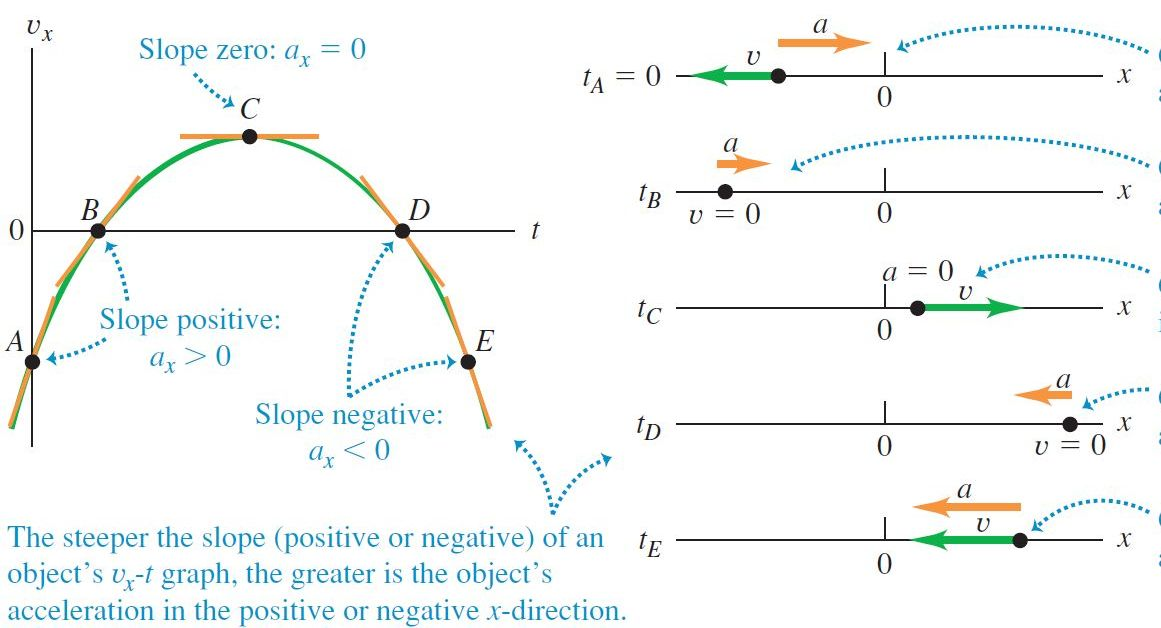
\includegraphics[width=1.\textwidth]{images/13.jpg}
   \caption{ {\tiny © University Physics 
   with Modern Physics, 13th Edition.} }
\end{figure}

 \end{frame}



%%%%%%%%%%%%%%%%%%%%%%%%%%%%%%%%%%%%%%%%%%%%%%%%%%%%%%%%%%%%%%%%%%%




\begin{frame}

Finding Acceleration on a x-t Graph 
\vspace{3mm}

  \begin{figure}[h!]   
   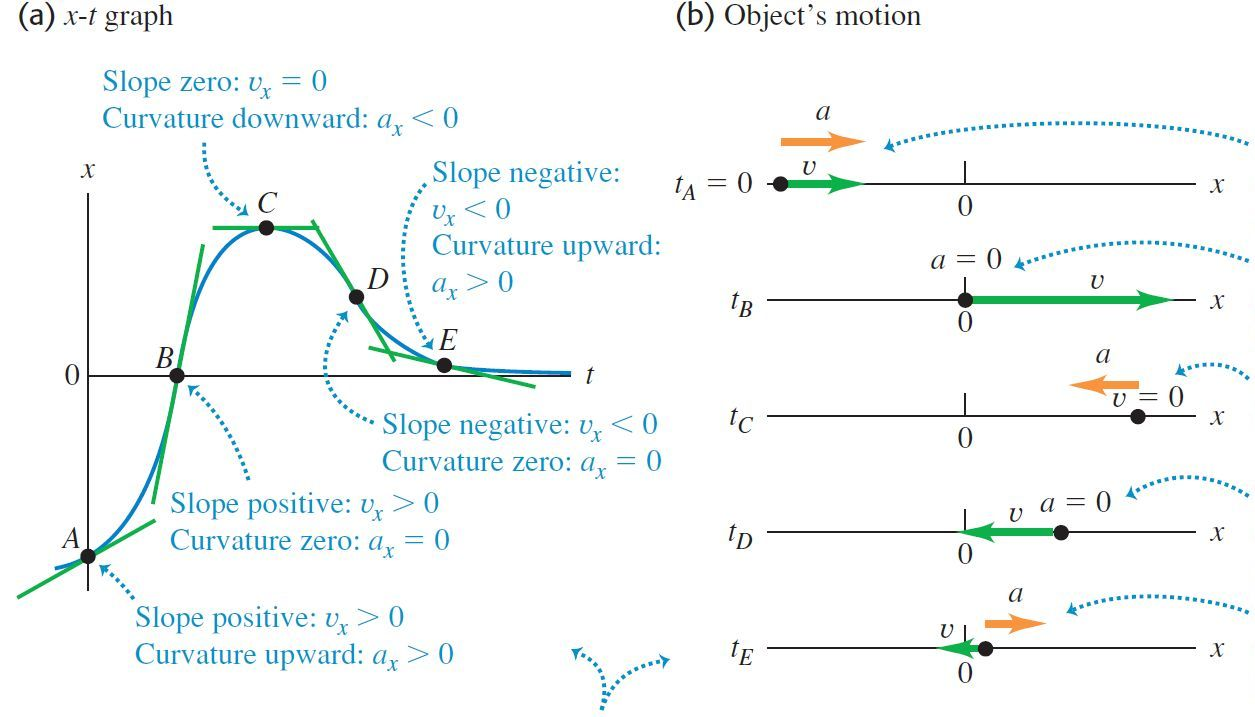
\includegraphics[width=1.1\textwidth]{images/14.jpg}
   \caption{ {\tiny © University Physics 
   with Modern Physics, 13th Edition.} }
\end{figure}

 \end{frame}



%%%%%%%%%%%%%%%%%%%%%%%%%%%%%%%%%%%%%%%%%%%%%%%%%%%%%%%%%%%%%%%%%%%




\begin{frame}

\begin{itemize}
\item If the curve is concave up, the acceleration is positive.
\pause
\item If the curve is concave dow, the aceleration is negative.
\pause
\item if the velocity has the same sign than the acceleration, the motion accelerated.
\pause
\item If the velocity has a opposite sign to the acceleration, the motion is decelerated.
\end{itemize}

 \end{frame}

%%%%%%%%%%%%%%%%%%%%%%%%%%%%%%%%%%%%%%%%%%%%%%%%%%%%%%%%%%%%%%%%%%%

\begin{frame}
Test your undertanding
\vspace{3mm}

   \begin{enumerate}
\item At which of the points P, Q, R, and S is the
x-acceleration positive?
\item At which points is the x-acceleration negative?
\item  At which points does the x-acceleration appear to be zero? 
\item At each point state
whether the velocity is increasing, decreasing, or not changing.

\end{enumerate}
   
   \begin{figure}[h!]   
   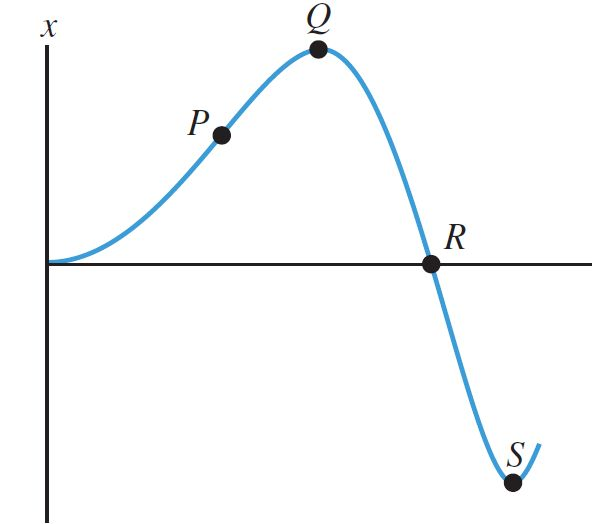
\includegraphics[width=0.4\textwidth]{images/10.jpg}
   \caption{ {\tiny © University Physics 
   with Modern Physics, 13th Edition.} }
\end{figure}

 \end{frame}



%%%%%%%%%%%%%%%%%%%%%%%%%%%%%%%%%%%%%%%%%%%%%%%%%%%%%%%%%%%%%%%%%%%
\subsection{Motion with Constant Acceleration}
%%%%%%%%%%%%%%%%%%%%%%%%%%%%%%%%%%%%%%%%%%%%%%%%%%%%%%%%%%%%%%%%%%%




\begin{frame}

   \begin{itemize}
      \item straight-line motion with constant
      acceleration
      \vspace{3mm}
      \pause
  
      \item the velocity changes at the same rate throughout the
      motion.
      \pause
         \begin{itemize}
           \item falling body when  the effects of the air are not important.
         \end{itemize}
   \end{itemize}
\end{frame}
%%%%%%%%%%%%%%%%%%%%%%%%%%%%%%%%%%%%%%%%%%%%%%%%%%%%%%%%%%%%%%%%%%%

\begin{frame}
   When the acceleration is constant,
   \vspace{3mm}
   \pause
   
   \begin{equation}
   a=\frac{v_2-v_1}{t_2-t_1}
   \end{equation}
   \pause
   \vspace{3mm}
   \pause
   if $t_1=0$, $v_1=v_0$ and $v_2=v$ $ \rightarrow v=at+v_0 $

   


   \begin{figure}[h!]
 
      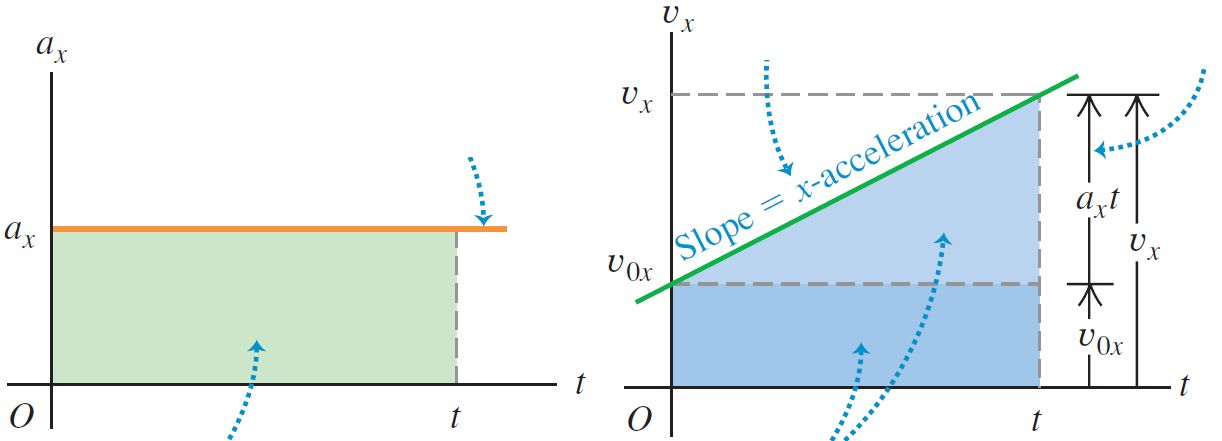
\includegraphics[width=0.8\textwidth]{images/15.jpg}
      \caption{ {\tiny © University Physics 
      with Modern Physics, 13th Edition.} }
    \end{figure}



 \end{frame}

%%%%%%%%%%%%%%%%%%%%%%%%%%%%%%%%%%%%%%%%%%%%%%%%%%%%%%%%%%%%%%%%%%%

\begin{frame}
   What is x(t)?
   \vspace{3mm}

   Let's use the expression for the average velocity,
\begin{equation*}
   v_{av}=\frac{x-x_0}{t}
\end{equation*}
When the acceleration is constant,  the average velocity is also

\begin{equation*}
   v_{av}=\frac{v+v_0}{2}
\end{equation*}

And..we already know that $v=at+v_0 $

Then\dots

\begin{equation}
   x=x_0+v_0t+\frac{1}{2}at^2
\end{equation}
 \end{frame}


 
%%%%%%%%%%%%%%%%%%%%%%%%%%%%%%%%%%%%%%%%%%%%%%%%%%%%%%%%%%%%%%%%%%%

\begin{frame}
   What is x(t)?
   \vspace{3mm}
Example: object motion, $v_0=0$ and $x_0=0$
   \begin{figure}[h!]
 
      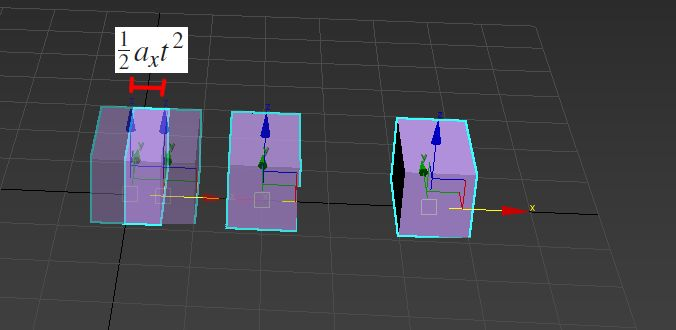
\includegraphics[width=0.8\textwidth]{images/16.jpg}
      \caption{ {\tiny © University Physics 
      with Modern Physics, 13th Edition.} }
    \end{figure}


 \end{frame}






 %%%%%%%%%%%%%%%%%%%%%%%%%%%%%%%%%%%%%%%%%%%%%%%%%%%%%%%%%%%%%%%%%%%

 \begin{frame}
  x(t) is a parababola
   \vspace{3mm}

   \begin{figure}[h!]
 
      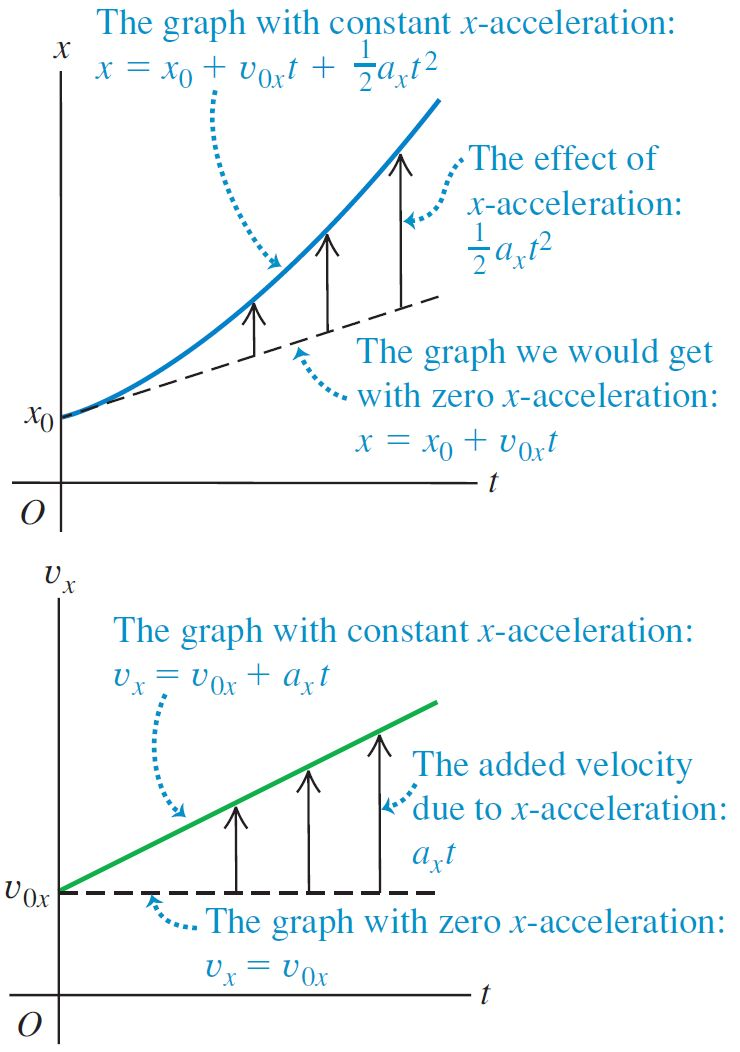
\includegraphics[width=0.4\textwidth]{images/18.jpg}
      \caption{ {\tiny © University Physics 
      with Modern Physics, 13th Edition.} }
    \end{figure}


 \end{frame}


  %%%%%%%%%%%%%%%%%%%%%%%%%%%%%%%%%%%%%%%%%%%%%%%%%%%%%%%%%%%%%%%%%%%

  \begin{frame}
 Example: Let's analyze the motion for the following graphs  
    \vspace{3mm}
 
    \begin{figure}[h!]
  
       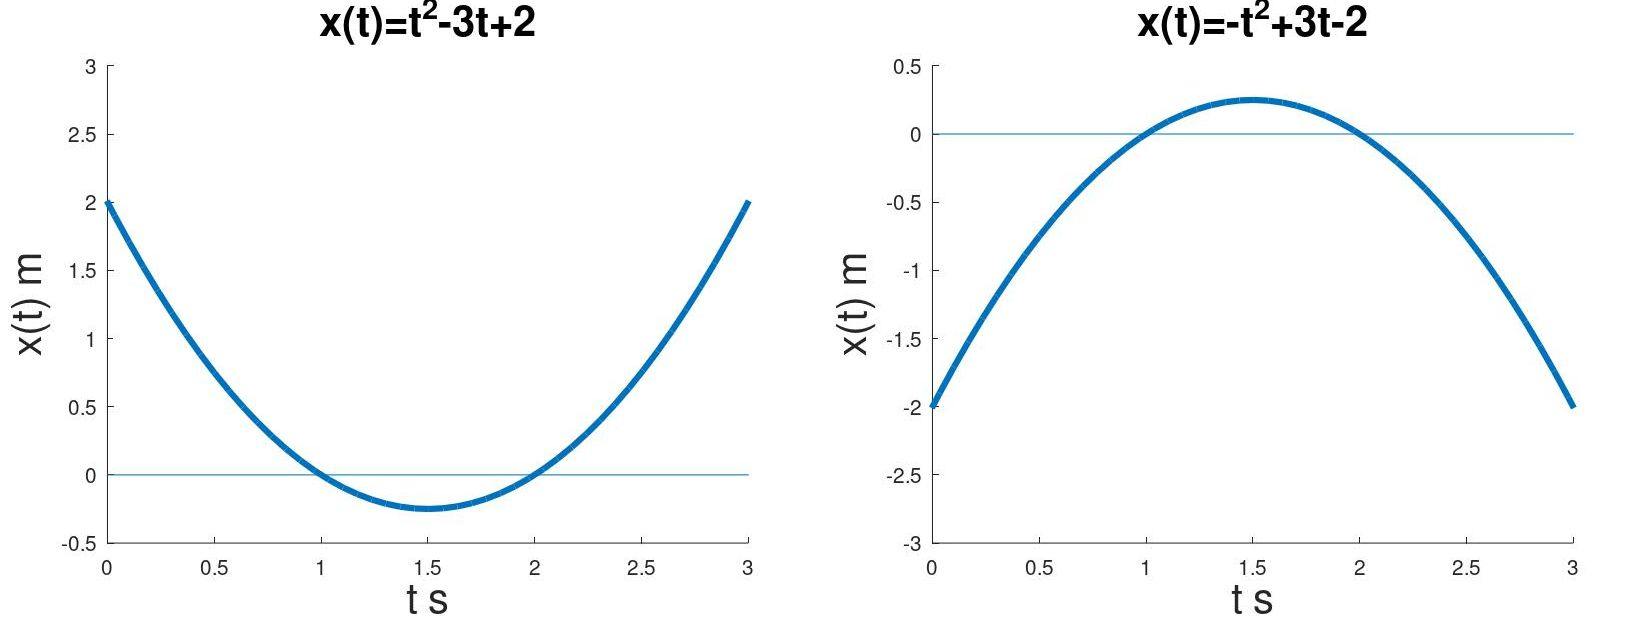
\includegraphics[width=1.\textwidth]{images/19.jpg}
       \caption{ {\tiny © University Physics 
       with Modern Physics, 13th Edition.} }
     \end{figure}
 
 
  \end{frame}
 
%%%%%%%%%%%%%%%%%%%%%%%%%%%%%%%%%%%%%%%%%%%%%%%%%%%%%%%%%%%%%%%%%%%

\begin{frame}
   DISCUSSION QUESTIONS
   \vspace{3mm}
   
   The top diagram in the figure represents a series of highspeed
photographs of an insect flying in a straight line from left to
right (in the positive x-direction). Which of the graphs of the bottom graphs 
most plausibly depicts this insect’s motion?

      \begin{figure}[h!]   
      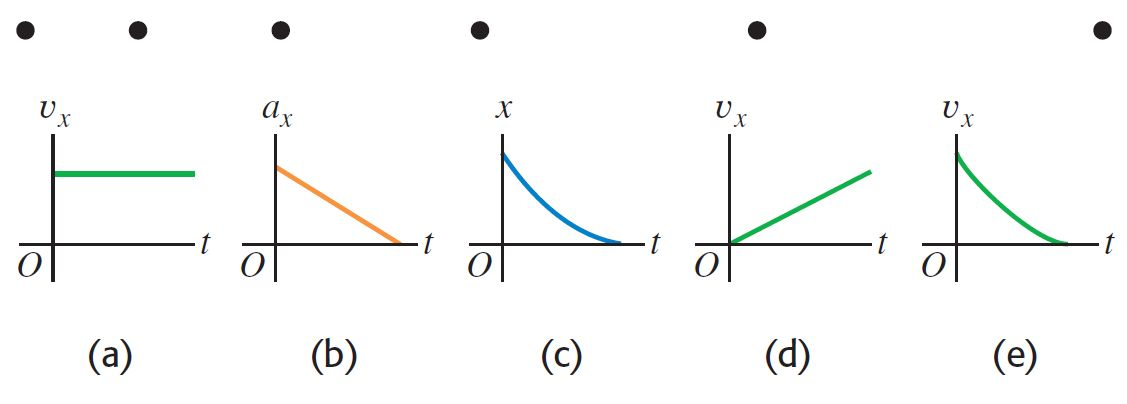
\includegraphics[width=0.8\textwidth]{images/21.jpg}
      \caption{ {\tiny © University Physics 
      with Modern Physics, 13th Edition.} }
   \end{figure}
   
    \end{frame}

  %%%%%%%%%%%%%%%%%%%%%%%%%%%%%%%%%%%%%%%%%%%%%%%%%%%%%%%%%%%%%%%%%%%

  \begin{frame}
 Another usefull expression valid for constant acceleration motion:
 
\begin{equation*}
   v=at+v_0 \rightarrow t=\frac{v-v_0}{a}
\end{equation*}
\pause

\begin{equation*}
  \rightarrow x=\frac{1}{2}a(\frac{v-v_0}{a})^2+v_0(\frac{v-v_0}{a})+x_0
\end{equation*}
\pause

\begin{equation*}
   \rightarrow x-x_0=\frac{v^2-v^2_0}{2a}
 \end{equation*}

  \end{frame}
 

 %%%%%%%%%%%%%%%%%%%%%%%%%%%%%%%%%%%%%%%%%%%%%%%%%%%%%%%%%%%%%%%%%%%

 \begin{frame}
   By using these equations, we can solve any
   problem involving straight-line motion of a particle with constant acceleration.
    \vspace{3mm}
 
    \begin{figure}[h!]
  
       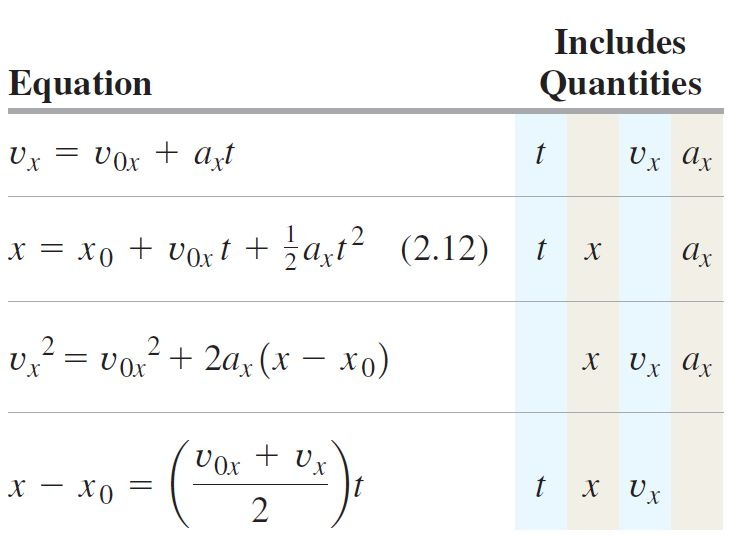
\includegraphics[width=0.65\textwidth]{images/equations1.jpg}
       \caption{ {\tiny © University Physics 
       with Modern Physics, 13th Edition.} }
     \end{figure}
 
 
  \end{frame}
 

  

 %%%%%%%%%%%%%%%%%%%%%%%%%%%%%%%%%%%%%%%%%%%%%%%%%%%%%%%%%%%%%%%%%%%

 \begin{frame}
  Exercise:
  \vspace{3mm}

  A motorist traveling with a constant speed of $15~m/s$ 
passes a school-crossing corner, where the speed limit is $10~m/s$.
 Just as the motorist passes the schoolcrossing
sign, a police officer on a motorcycle stopped there starts
in pursuit with a constant acceleration of $3~m/s^2$

\begin{enumerate}
   \item How much time elapses before the officer passes the motorist?
   \item What is the officer’s speed at that time?
   \item At that time, what distance has each vehicle traveled?
\end{enumerate}

 
 
  \end{frame}


 %%%%%%%%%%%%%%%%%%%%%%%%%%%%%%%%%%%%%%%%%%%%%%%%%%%%%%%%%%%%%%%%%%%

 \begin{frame}
  Testing your understanding
  \vspace{3mm}
\begin{itemize}
   \item Can an object with constant acceleration reverse its direction
   of travel? Can it reverse its direction twice?
   \item Under what conditions is average velocity equal to instantaneous
   velocity?
   \item Is it possible for an object to be slowing down while its
   acceleration is increasing in magnitude?
   \item  To be speeding up
   while its acceleration is decreasing? +98
\end{itemize}

 
  
  
   \end{frame}















%%%%%%%%%%%%%%%%%%%%%%%%%%%%%%%%%%%%%%%%%%%%%%%%%%%%%%%%%%%%%%%%%%%
 \end{document}
%%%%%%%%%%%%%%%%%%%%%%%%%%%%%%%%%%%%%%%%%%%%%%%%%%%%%%%%%%%%%%%%%%%